\section*{Part 3}
Figure \ref{fig:avg_em} illustrates the relationship between temperature and two key properties magnetization and energy for different sizes of square lattices in the 2D Ising model.\\
\\
The left column presents the average absolute magnetization as a function of temperature. In each plot, we observe that the steepest change in magnetization, indicating the phase transition, occurs near the critical temperature, $T_c \approx 2.269$\\
\\
Furthere observations on Magnetization are:
\begin{itemize}
	\item All three lattice sizes exhibit a similar pattern: for low temperatures $T<1$, the system remains in an ordered state with high and stable magnetization, as most spins align in the same direction.
	\item The most significant drop in magnetization occurs in the critical region between $T= 2.0$and $T= 2.5$ for all lattice sizes, aligning with the expected phase transition at $T_c$. The transition becomes steeper for larger lattices, indicating a sharper phase transition as the system size increases. 
	\item For temperatures $T>2.5$, magnetization continues to decrease but at a much slower rate. As $T$ increases beyond $3.0$, the system approaches complete randomness, leading to near-zero magnetization. \end{itemize}
The right column displays the average energy as a function of temperature. We can make the following observations on Energy:
\begin{itemize} 
	\item For $T<1$, all systems remain at their minimum energy state, corresponding to a highly ordered configuration.
	\item As temperature increases $T>1.5$, the spins start to misalign with their neighbors due to increased thermal fluctuations. This occurs as thermal energy begins to overcome the exchange coupling $J$, leading to the disruption of ordered spin states. 
	\item At even higher temperatures, the system gradually approaches maximum disorder, with energy increasing toward zero. \end{itemize}
The data clearly demonstrates a phase transition near the critical temperature, showcasing the classical behavior of the 2D Ising model. As the system transitions from a low-temperature ordered state to a high-temperature disordered state, we observe a sharp drop in magnetization and a corresponding increase in energy, particularly for larger lattice sizes.
\begin{figure}[t]
	\centering
	\begin{subfigure}{0.5\textwidth}
		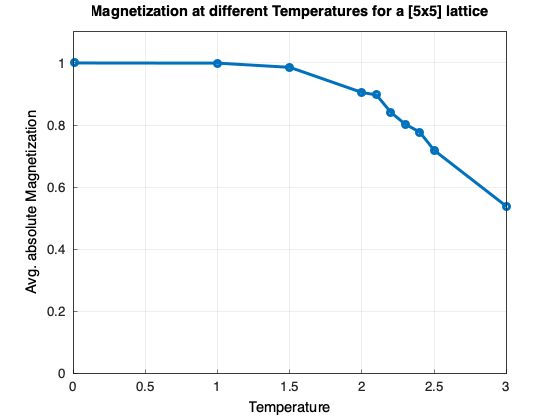
\includegraphics[width=\textwidth]{./img/avg_mag_5.png}
		\caption{$L=[5\times5]$}
		\label{sfig:sublabel1}
	\end{subfigure}%
	~
	\begin{subfigure}{0.5\textwidth}
		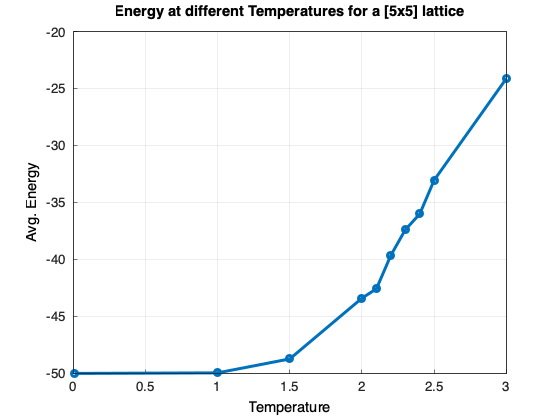
\includegraphics[width=\textwidth]{./img/avg_en_5.png}
		\caption{$L=[5\times5]$}
		\label{sfig:sublabel2}
	\end{subfigure}\\
	\begin{subfigure}{0.5\textwidth}
		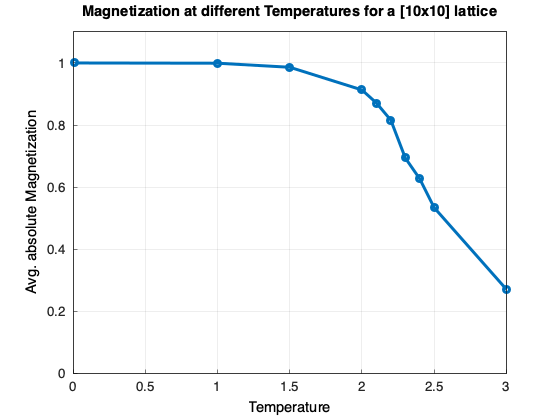
\includegraphics[width=\textwidth]{./img/avg_mag_10.png}
		\caption{$L=[10\times10]$}
		\label{sfig:sublabel3}
	\end{subfigure}%
	~
	\begin{subfigure}{0.5\textwidth}
		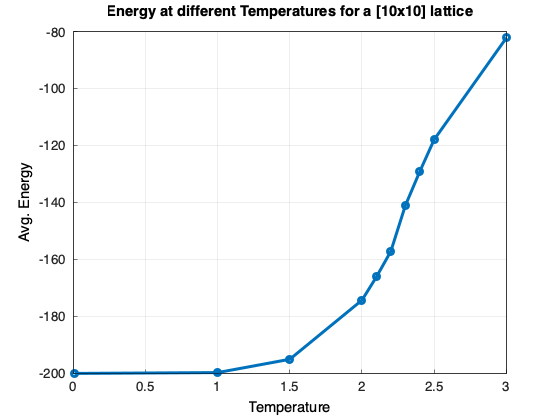
\includegraphics[width=\textwidth]{./img/avg_en_10.png}
		\caption{$L=[10\times10]$}
		\label{sfig:sublabel4}
	\end{subfigure}\\
	\begin{subfigure}{0.5\textwidth}
		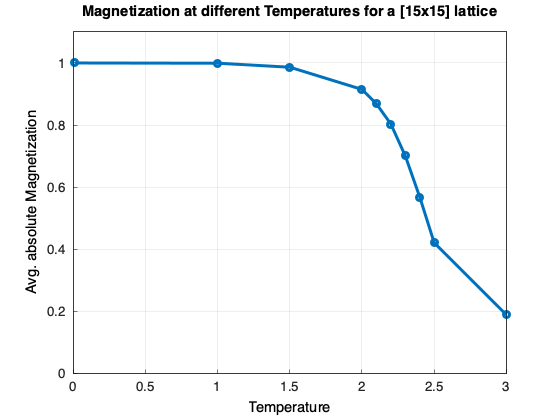
\includegraphics[width=\textwidth]{./img/avg_mag_15.png}
		\caption{$L=[15\times15]$}
		\label{sfig:sublabel5}
	\end{subfigure}%
	~
	\begin{subfigure}{0.5\textwidth}
		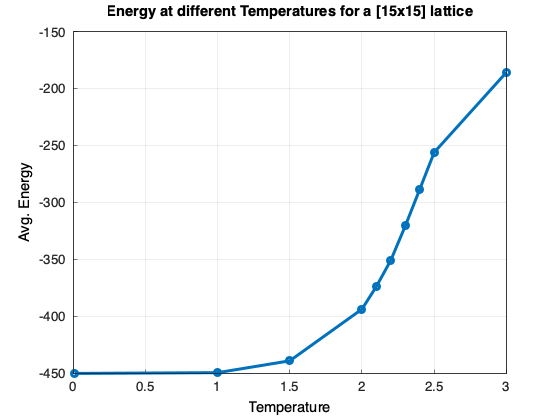
\includegraphics[width=\textwidth]{./img/avg_en_15.png}
		\caption{$L=[15\times15]$}
		\label{sfig:sublabel6}
	\end{subfigure}

	\caption{\textbf{Markov Chains}
		Average absolute magnetization at different temperature is plotted on the left, while on the right the average Energy is plotted versus the temperature.
	}
	\label{fig:avg_em}
\end{figure}
\begin{figure}[t]
	\centering
	\begin{subfigure}{0.5\textwidth}
		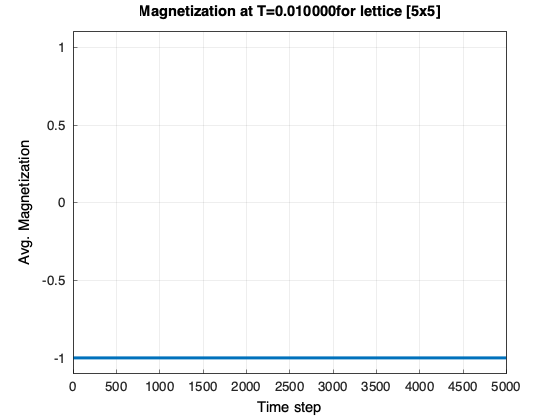
\includegraphics[width=\textwidth]{./img/mag_time_0.010000_5.png}
		\caption{$T=0.01$}
		\label{sfig:p1}
	\end{subfigure}%
	~
	\begin{subfigure}{0.5\textwidth}
		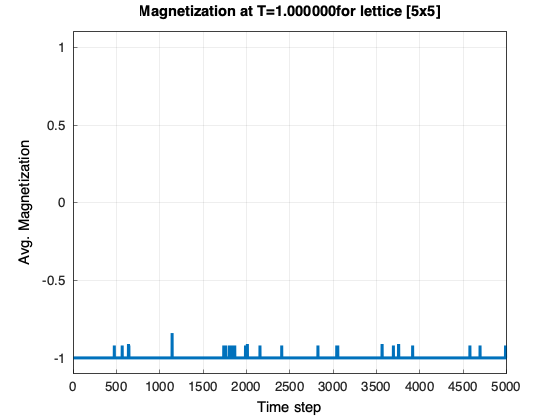
\includegraphics[width=\textwidth]{./img/mag_time_1.000000_5.png}
		\caption{$T=1.0$}
		\label{sfig:p2}
	\end{subfigure}\\
	\begin{subfigure}{0.5\textwidth}
		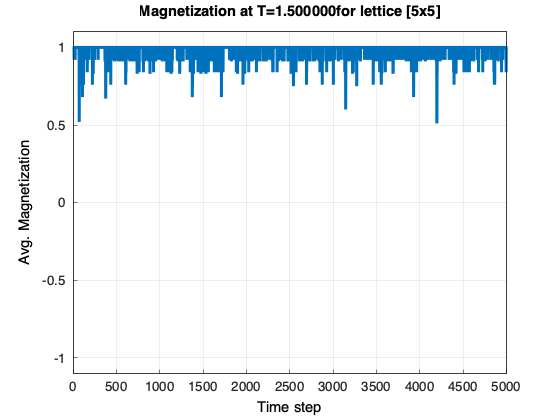
\includegraphics[width=\textwidth]{./img/mag_time_1.500000_5.png}
		\caption{$T=1.5$}
		\label{sfig:p3}
	\end{subfigure}%
	~
	\begin{subfigure}{0.5\textwidth}
		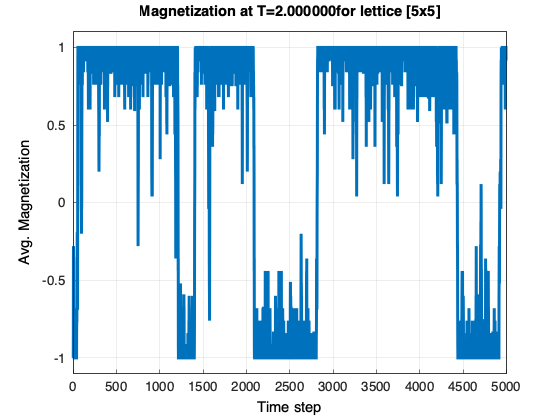
\includegraphics[width=\textwidth]{./img/mag_time_2.000000_5.png}
		\caption{$T=2.0$}
		\label{sfig:p4}
	\end{subfigure}\\
	\begin{subfigure}{0.5\textwidth}
		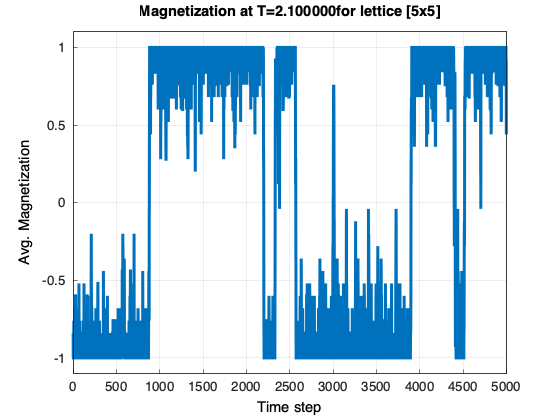
\includegraphics[width=\textwidth]{./img/mag_time_2.100000_5.png}
		\caption{$T=2.1$}
		\label{sfig:p5}
	\end{subfigure}%
	~
	\begin{subfigure}{0.5\textwidth}
		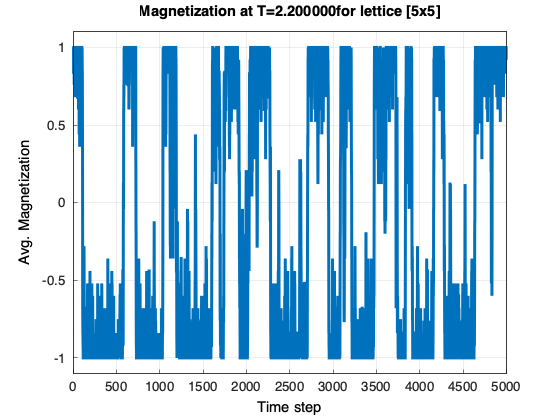
\includegraphics[width=\textwidth]{./img/mag_time_2.200000_5.png}
		\caption{$T=2.2$}
		\label{sfig:p6}
	\end{subfigure}%

	\caption{\textbf{Dependence of $M$ on the simulation time at temperature $T < T_C$}
	}
	\label{fig:mag_time}
\end{figure}
The plots in Figure~\ref{fig:mag_time} depict the evolution of magnetization over time for an $5 \times 5$ Ising model lattice at different temperatures. Each system was initialized randomly, meaning the overall sign of magnetization may vary between subfigures (e.g., Subfigure~\ref{sfig:p3} compared to \ref{sfig:p1} or \ref{sfig:p2}).
The following key observation can be made on Magnetization and Sign Flipping:

\begin{itemize}
	\item Subfigure~\ref{sfig:p1} ($T=0.01$): At temperatures very close to zero, the system is fully ordered, with magnetization staying at $-1$ (or $1$) throughout the entire simulation. No sign flips occur, as thermal energy is insufficient to disrupt spin alignment.
\item Subfigure~\ref{sfig:p2} ($T=1.0$): The system remains predominantly magnetized in one direction, but small fluctuations appear. However, no full sign flips are observed.
\item Subfigure~\ref{sfig:p3} ($T=1.5$): Larger deviations in magnetization occur, yet the system still retains a dominant direction. No complete sign flips are observed, though fluctuations increase.
\item Subfigures~\ref{sfig:p4}, \ref{sfig:p5}, and \ref{sfig:p6} ($T=2.0,2.1,2.2$): As temperature increases and approaches the critical temperature $T_c$, magnetization fluctuates more violently. Frequent sign flips occur, indicating the system oscillates between states with positive and negative magnetization due to increasing thermal energy. These fluctuations become more pronounced closer to $T_c$, as thermal agitation competes with spin alignment.
\end{itemize}

